% Chapter Template

\chapter{Activity--Rotation--Age Investigation} % Main chapter title

\label{Chapter5} 

\epigraph{\itshape Sometimes the wheel turns slowly, but it turns.}{---Lorne Michaels}

\section{Introduction}

The work I presented in Chapters \ref{Chapter3} and \ref{Chapter4} investigated the age--activity relationship through coronal and chromospheric emission for stars older than a gigayear. Chapter \ref{Chapter3} \citep{Booth_etal_2017} showed that the X-ray luminosity--age relationship steepens for older stars when compared to younger cluster stars. Chapter \ref{Chapter4} presented the chromospheric emission (\Rprime) for a sample of FG--type stars and found that, even when mass and metallicity is taken into account, the sample displayed lower chromospheric activity than expected.

However, the age--activity relationship is a consequence of the magnetic braking that removes angular momentum from the star on the main sequence. Thus, the age--activity relationship is inherently linked to the rotational evolution. As discussed in Section \ref{Chp2_activity-rotation_lit_review}, this has led to studies on the activity-rotation relationship (see e.g. \citealt{Pizzolato_etal_2003,Wright_etal_2011}). Given the reports of weakened magnetic braking for stars of a similar age \citep{van_Saders_etal_2016}, it is also important to consider the stellar rotation periods. The work presented in this chapter aims to collect rotation periods for the sample of stars I presented in Chapters \ref{Chapter3} and \ref{Chapter4} and investigate the activity--rotation and rotation--age relationships.

\subsection{Determining rotation periods}
\label{Chp5_Prot_methods}

There are several possible methods to determine the rotation period of a star: Since the rotation periods considered in this work were collected from literature using various methods, they are summarised here for convenience.

\paragraph{Photometric variability}
This may be the most common method of determining the rotation period for a star. As discussed in Section \ref{Chp1_photosphere}, starspots are observed in light curves as quasi-periodic variations in the brightness of star as the starspot rotates in and out of view of the observer. One common technique of determining the rotation period from photometric variability is the Lomb-Scargle periodogram \citep{Lomb_1976,Scargle_1982}, which uses a Fourier transform to search for periodicities of a sinusoidal nature. Typically, a distribution of peaks will appear in the power spectrum and the period with the largest Lomb-Scargle power will correspond to the rotation period. This is a commonly used technique to determine the stellar rotation period (see e.g. \citealt{do_Nascimento_etal_2014,Nielsen_etal_2013}).

Another technique used to determine periodic variations in light curve is the autocorrelation function (ACF): This method determines how correlated the light curve is with itself when offset by a certain time lag. This can be performed for a range of time lags with repeated spot crossings, providing peaks in the ACF at time periods associated with the rotation period. An advantage of this method is that the shape of the periodicity in the light curve is not assumed and thus may be more useful in cases where the modulation is not perfectly sinusoidal. This technique is also fairly common in the literature and has been used for large samples of stars from \textit{Kepler} \citep{McQuillan_etal_2014}.

\paragraph{Magnetic activity indicators}
Magnetic activity indicators such as calcium emission from the \caII lines or X-ray luminosity can also be used to determine the stellar rotation period. Since these activity indicators are sensitive to regions of magnetic activity (such as starspots and/or plage) on the stellar surface, as the regions rotate in and out of view this will leave a rotational modulation in the magnetic activity indicator. Therefore, this method of determining the rotation period requires observations sampled over the timescale of several rotation periods. These observations can then be analysed in a similar fashion to those from photometric variability, e.g. by using a Lomb-Scargle periodogram. This technique is ideal for stars with more subtle photometric variation, for example slower rotators. Examples of this method in the literature include \citet{DeWarf_etal_2010,Robertson_etal_2015_GJ176,Boro_Saikia_etal_2016,Hempelmann_etal_2016}. It is important to note that using photometric and magnetic activity variability as a method of determining the stellar rotation period requires an inhomogeneous distribution of magnetic activity regions on the stellar surface.

\paragraph{Asteroseismology}
As discussed in Section \ref{Section:intro_ages}, asteroseismology is a valuable tool for determining fundamental parameters through observations of stellar oscillations. However, any departure from solid body rotation will result in a frequency splitting of non-radial p modes known as rotational splitting. From helioseismology, the analysis of the rotational splitting has provided detail about the interior of the Sun and revealed the presence of the tachocline \citep{Spiegel_Zahn_1992}, which is instrumental in stellar dynamo theory. However, in order to obtain rotational splitting from asteroseismology, data sets with timescales on the order of years are required (e.g. \citealt{Davies_etal_2015}). This is due to the amplitude of the rotational splitting, which varies from a few micro-Hertz for more massive or younger stars down to a fraction of a micro-Hertz for less massive or older stars. The rotational splitting of p modes in solar-like oscillators are predominantly determined by the rotational profile in the stellar envelope. This is important to note as it is not necessarily the same as the surface rotation period and there is still some debate in the literature about the accuracy of asteroseismic rotation periods (see e.g. \citealt{Barnes_etal_2016_aspect_gyro}).

\section{Data}
\label{Chp5_data}

The sample of stars considered in this analysis comes from the X-ray luminosity and calcium emission studies that I conducted in Chapters \ref{Chapter3} and \ref{Chapter4}. Rotation periods for my sample of stars were searched for in the literature using the online service \textit{VizieR}\footnote{\href{http://vizier.u-strasbg.fr/viz-bin/VizieR}{http://vizier.u-strasbg.fr/viz-bin/VizieR}} \citep{Ochsenbein_etal_2000}. In addition to this, literature values for the \Rprime activity indicator were collected for the sample of stars from the X-ray luminosity study. In total, 29 stars with rotation periods are considered in this analysis covering a range of spectral types from F--type to M--type; 21 of these stars have values for the \Rprime indicator and 20 stars have values for the X-ray luminosity. Note that for the stars with X-ray luminosities, 8 are upper limit results. The details of the literature values collected and the relevant references for the sample of stars are shown in Appendix \ref{App_I_activity_rotation}. Note that where literature rotation periods did not have associated errors, a standard error of 0.5 days was used.

Since the sample of stars considered in this work is small, comparison samples from previous activity--rotation studies were also used. To compare the stars with values for the \Rprime indicator to stars of a similar age, the sample of stars from \citet{Metcalfe_etal_2016} (henceforth M16) was used. Data were also taken from \citet{Baliunas_etal_1996} (henceforth B96) to compare the \Rprime samples from this work and M16. For the X-ray sample, data were taken from \citet{Wright_etal_2011} (W11) to compare against the sample from my own work.

\subsection{Consistency of \texorpdfstring{$P_{rot}$}{Prot}}
For a number of stars in the sample, several sources were found for the rotation period in the literature. In this section I will discuss the consistency of the rotation periods found in the literature. Note that there are error bars associated with the majority of the values discussed below and they are recorded in Appendix \ref{App_I_activity_rotation}.

\textit{61 Cyg A}: The rotation period used in this work stems from \citet{Boro_Saikia_etal_2016} and has a value of $35.70$~days. This rotation period was derived from chromospheric activity measurements. Three earlier studies that used the same technique \citep{Vaughan_etal_1981,Hallam_Wolff_1981,Donahue_etal_1996} also have values consistent with the rotation period used in this work.

\textit{61 Cyg B}: The rotation period used in this work comes from \citet{Vaughan_etal_1981} and has a value of $48.0$~days. This value is in agreement with the value found from \citet{Hallam_Wolff_1981}. However, a much shorter rotation period is reported in \citet{Donahue_etal_1996} of $37.84$~days. This is an average rotation period calculated from a number of observations, where the range of the rotation periods observed span from $31.78$ to $46.57$~days. Since all of these studies rely on the the measurement of chromospheric emission, the variation in the rotation period may be due to active regions on varying stellar latitudes.

\textit{GJ 176}: This stellar rotation period originates from \citet{Robertson_etal_2015_GJ176} and has a value of $39.46$~days. This rotation period was derived from stellar photometric observations. An additional rotation period was found in \citet{Kiraga_Stepien_2007}, which also used photometric variability and found a rotation period consistent with the value used in this work.

\textit{HR 7703}: This stellar rotation period comes from \citet{Ammler_vonEiff_Reiners_2012} and has a minimum value of $17.1$~days. This rotation period is derived from spectral line broadening; the true rotation period will be larger than this, since the stellar inclination is unknown. An erroneous rotation period is reported in \citet{Pizzolato_etal_2003} of $45.0$~days. This rotation period stems from \citet{Saar_etal_1997} and was estimated from the overall \caII emission level, not periodic variations in the emission.

\textit{KIC 10016239 and KIC 3123191}: The stellar rotation periods used in this work stems from \citet{McQuillan_etal_2014} and have values of $4.89$ and $20.55$~days, respectively. These values are calculated from photometric variation in light curves. \citet{Garcia_etal_2014} also used photometric variation to determine the rotation period for these two stars and found values that are in agreement with the values used in this work.

\textit{KIC 9955598}: The rotation period used in this work originates from \citet{Garcia_etal_2014} and has a value of $34.2$~days. \citet{Garcia_etal_2014} used photometric variation to derive rotation periods. \citet{Paz_Chinchon_etal_2015} also derived a rotation period using photometric variation and found a value for the rotation period of $20.1$~days. However, this was flagged as a lower probability rotation period by \citet{Paz_Chinchon_etal_2015} as it did not exhibit clear semi-sinusoidal signatures, therefore the rotation period from \citet{Garcia_etal_2014} was used in this work. 

\textit{Proxima Centauri}: The stellar rotation period comes from \citet{Collins_etal_2017} and has a value of $82.6$~days. This rotation period is calculated from the variability of the \Halpha index. The rotation period is also consistent with the photometric variation as calculated using the Hubble Space Telescope \citep{Benedict_etal_1998}.

\textit{KIC 10454113}: The rotation period stems from \citet{McQuillan_etal_2014} and has a value of $14.45$~days. Consistent values for the rotation period for this star are also found in \citet{do_Nascimento_etal_2014} and \citet{Nielsen_etal_2013}.

\textit{KIC 10963065}: The stellar rotation period used in this work originates from \citet{Paz_Chinchon_etal_2015} with a value of $12.96$~days. Similar values for the rotation period were also found in \citet{McQuillan_etal_2013} and \citet{Mazeh_etal_2015}.

\textit{KIC 7206837}: The stellar rotation period comes from \citet{McQuillan_etal_2014} and has a value of $4.07$~days. This value is consistent with the rotation period found in \citet{Nielsen_etal_2013}.

\textit{KIC 9139163}: This star had only one source for the rotation period in the literature \citep{Janes_2017}; however, the rotation period was reported to be $0.61$~days. This is the shortest period found for the sample of stars considered in this work, hence why it is highlighted here. Unfortunately, no other sources reported a rotation period for this star, therefore it is not possible to determine if this is an erroneous value.

\section{Method}
\label{Chp5_method}

As discussed in Section \ref{Chp2_activity-rotation_lit_review}, the activity--rotation relationship is usually calibrated in terms of Rossby number (\Ro). \Ro is defined as the as the rotation period divided by the convective turnover time (\tauc). In this work, \tauc was calculated using the relations from W11 that were derived empirically. Here, I will summarise the method W11 used to empirically derive the relationship between colour/mass and \tauc.

By using an empirical method, it assumes that the activity--rotation relationship can be divided into saturated and non-saturated regimes. This assumption is well--supported by the literature to date (see Section \ref{Chp2_activity-rotation_lit_review}). W11 divided their sample into bins of $B-V$ colour with approximately equal number of stars in each bin. Note that the $B-V$ colour is a proxy for mass and will be referred to as a mass bin. For each mass bin, the activity--rotation relationship was fitted with Equation \ref{Eq:W11_tauc_method_fit_eq} where $\frac{L_{x}}{L_{BOL}}$ is the ratio of X-ray to bolometric luminosity, $C_{B-V}$ is a colour dependent constant, $P_{sat}$ is the rotation period that divides the saturated and non-saturated regimes, and $\frac{L_{x}}{L_{BOL}})_{sat}$ is the X-ray to bolometric luminosity ratio in the saturated regime. The parameters $(\frac{L_{x}}{L_{BOL}})_{sat}$ and $P_{sat}$ are fitted for each of the mass bins using the $\beta$ value found in W11.

\begin{equation}
    \frac{L_{x}}{L_{BOL}} = 
    \begin{cases}
        C_{B-V}P_{rot}^{\beta} & P_{rot} > P_{sat} \\
        (\frac{L_{x}}{L_{BOL}})_{sat} & P_{rot} < P_{sat}
    \end{cases}
    \label{Eq:W11_tauc_method_fit_eq}
\end{equation}

The fits from each mass bins were used by W11 to determine the colour--dependent constant ($C_{B-V}$). The colour--dependent constant is defined in Equation \ref{Eq:W11_tauc_method_CBV} where $C$ is the scaling constant. W11 found the colour dependence by setting $C$ so that the \tauc value for solar-mass stars matched the values from \citet{Noyes_etal_1984}. This allowed for \tauc to be plotted as a function of colour and/or mass and the best-fitting relationship to be found. The best-fitting relationships are shown in Equation \ref{Eq:W11_tauc_VK}, where X is equal to $V-K$ and is valid in the range: $1.1 < V-K < 6.6$, and Equation \ref{Eq:W11_tauc_mass}, where $M/M_{\odot}$ is the stellar mass in terms of solar mass. These two equations are used to calculate \tauc for the sample of stars considered in this analysis.

\begin{equation}
    C_{B-V} = C\tau_{c}^{-\beta}
    \label{Eq:W11_tauc_method_CBV}
\end{equation}

\begin{equation}
    \log \tau_{c} = 
    \begin{cases}
        0.73 + 0.22X & X < 3.5 \\
        -2.16 +1.50X - 0.13X^{2} & X > 3.5
    \end{cases}
    \label{Eq:W11_tauc_VK}
\end{equation}

\begin{equation}
    \log \tau_{c} = 1.16 - 1.49\log(M/M_{\odot}) - 0.54\log^{2}(M/M_{\odot})
    \label{Eq:W11_tauc_mass}
\end{equation}

\begin{table}[t]
\centering
\begin{tabular}{lccc}
\hline
Spectral Type & $B-V$   & $V-K$  & $T_{eff}$ \\
\hline
F1V        & 0.343 & 0.850  & 7030 \\
F2V        & 0.374 & 0.925 & 6810 \\
F3V        & 0.389 & 0.961 & 6720 \\
F4V        & 0.412 & 1.017 & 6640 \\
F5V        & 0.438 & 1.079 & 6510 \\
F6V        & 0.484 & 1.185 & 6340 \\
F7V        & 0.510  & 1.244 & 6240 \\
F8V        & 0.530  & 1.290  & 6150 \\
F9V        & 0.552 & 1.340  & 6040 \\
G0V        & 0.588 & 1.421 & 5940 \\
G1V        & 0.604 & 1.458 & 5880 \\
G2V        & 0.642 & 1.545 & 5780 \\
G3V        & 0.661 & 1.59  & 5700 \\
G4V        & 0.674 & 1.621 & 5640 \\
G5V        & 0.680  & 1.635 & 5620 \\
G6V        & 0.704 & 1.693 & 5580 \\
G7V        & 0.713 & 1.712 & 5520 \\
G8V        & 0.737 & 1.768 & 5490 \\
G9V        & 0.777 & 1.861 & 5340 \\
\hline
\end{tabular}
\caption[\citet{Pecaut_etal_2012} table for colour conversion]{Part of Table 3 from \citet{Pecaut_etal_2012} used to convert $B-V$ into $V-K$. See Section \ref{Chp5_method}}
\label{Pecaut_table3}
\end{table}

For the majority of the stars considered in this analysis, masses were available either from asteroseismology or the literature. Therefore, \tauc was calculated using Equation \ref{Eq:W11_tauc_mass}. However, for the sample of stars from B96, no masses were available. Therefore, Table 3 from \citet{Pecaut_etal_2012} (shown in Table \ref{Pecaut_table3}) was used to convert $B-V$ values into $V-K$ values for this sample of stars and Equation \ref{Eq:W11_tauc_VK} was used to calculate \tauc. Since the table from \citet{Pecaut_etal_2012} is limited to $B-V < 0.77$, the sample from B96 was also limited to stars that fell into this range.

\section{Results}

\subsection{Activity--rotation}
\label{Chp5_results_activity_rotation}

\begin{figure}[!ht]
    \centering
    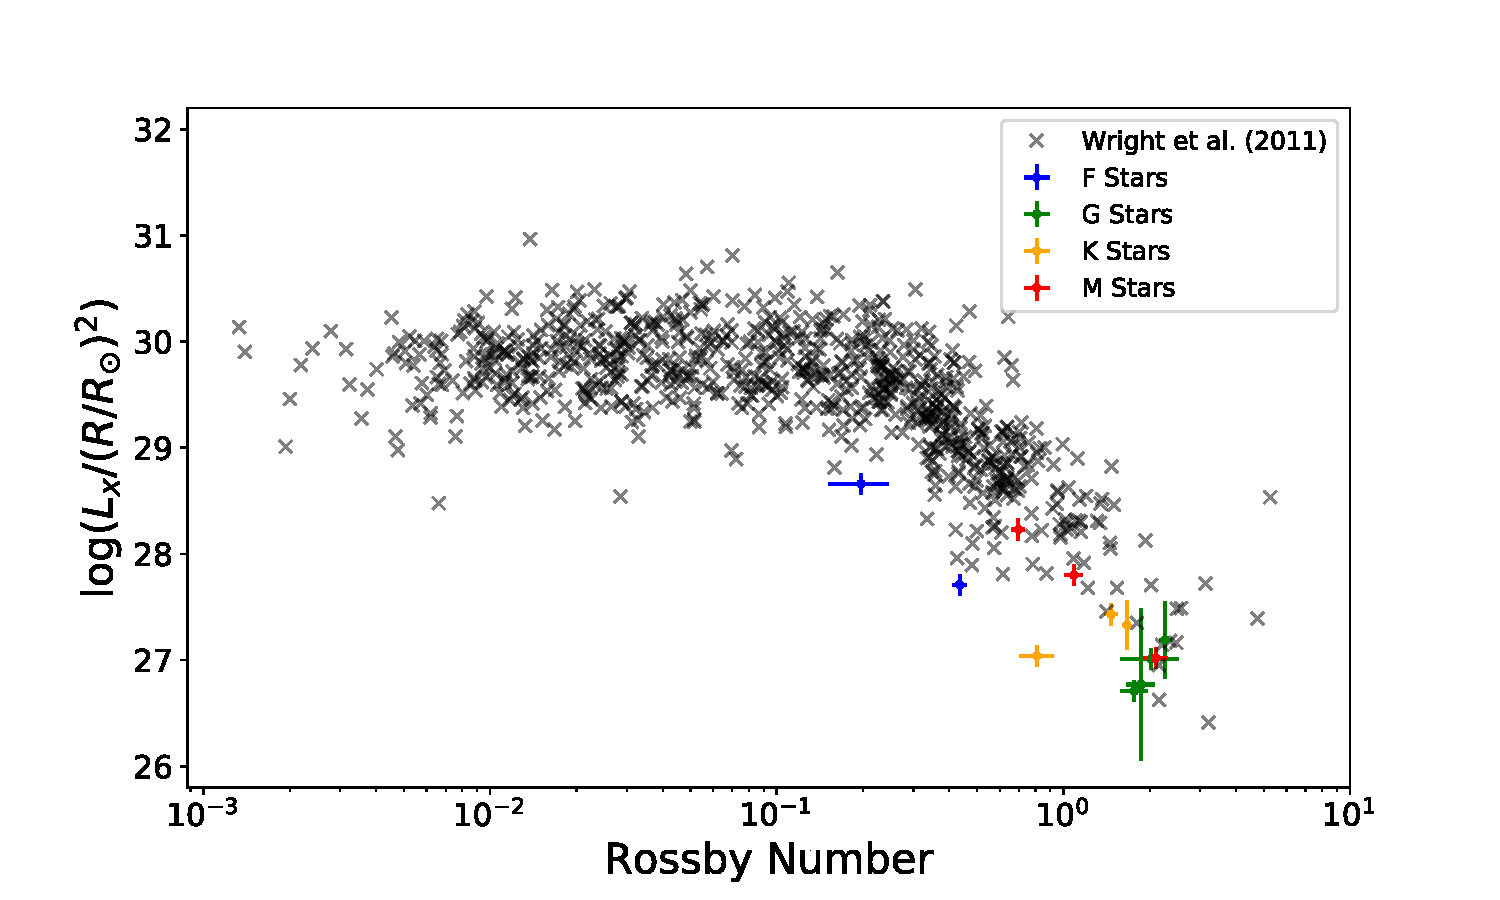
\includegraphics[width=0.95\textwidth]{Figures/5-Activity_rotation/lx_v_R0.pdf}
    \caption[$L_{x}$ as a function of \Ro]{X-ray luminosity normalised by stellar surface area as a function of \Ro for the sample of stars from the X-ray study with literature rotation periods. The sample from \citet{Wright_etal_2011} is plotted for comparison.}
    \label{fig:lx_v_ro}
\end{figure}

Twelve stars from the X-ray study \citep{Booth_etal_2017} with determined X-ray luminosities (i.e. not upper limit results) were found to have rotation periods in the literature. This stellar sample is plotted as a function of \Ro alongside the W11 sample of stars as shown in Figure \ref{fig:lx_v_ro}. This plot shows that the sample of old, inactive stars generally lie in the unsaturated regime of the activity--rotation relationship, as expected. However, my sample tends to lie on the lower activity end of the scatter in the activity--rotation relationship. This is to be expected, since the sample of stars considered in this work are old and inactive stars. However, the majority of stars in the sample are in agreement with the W11 sample, suggesting that, even at these older ages, the stellar magnetic activity and rotation are still inherently linked. Therefore, magnetic activity and rotation should show similar trends with stellar age. The exception to this is the two F--type stars that lie below the W11 sample. This will be discussed in more detail in Section \ref{Chp5_discussion}.

\begin{figure}
    \centering
    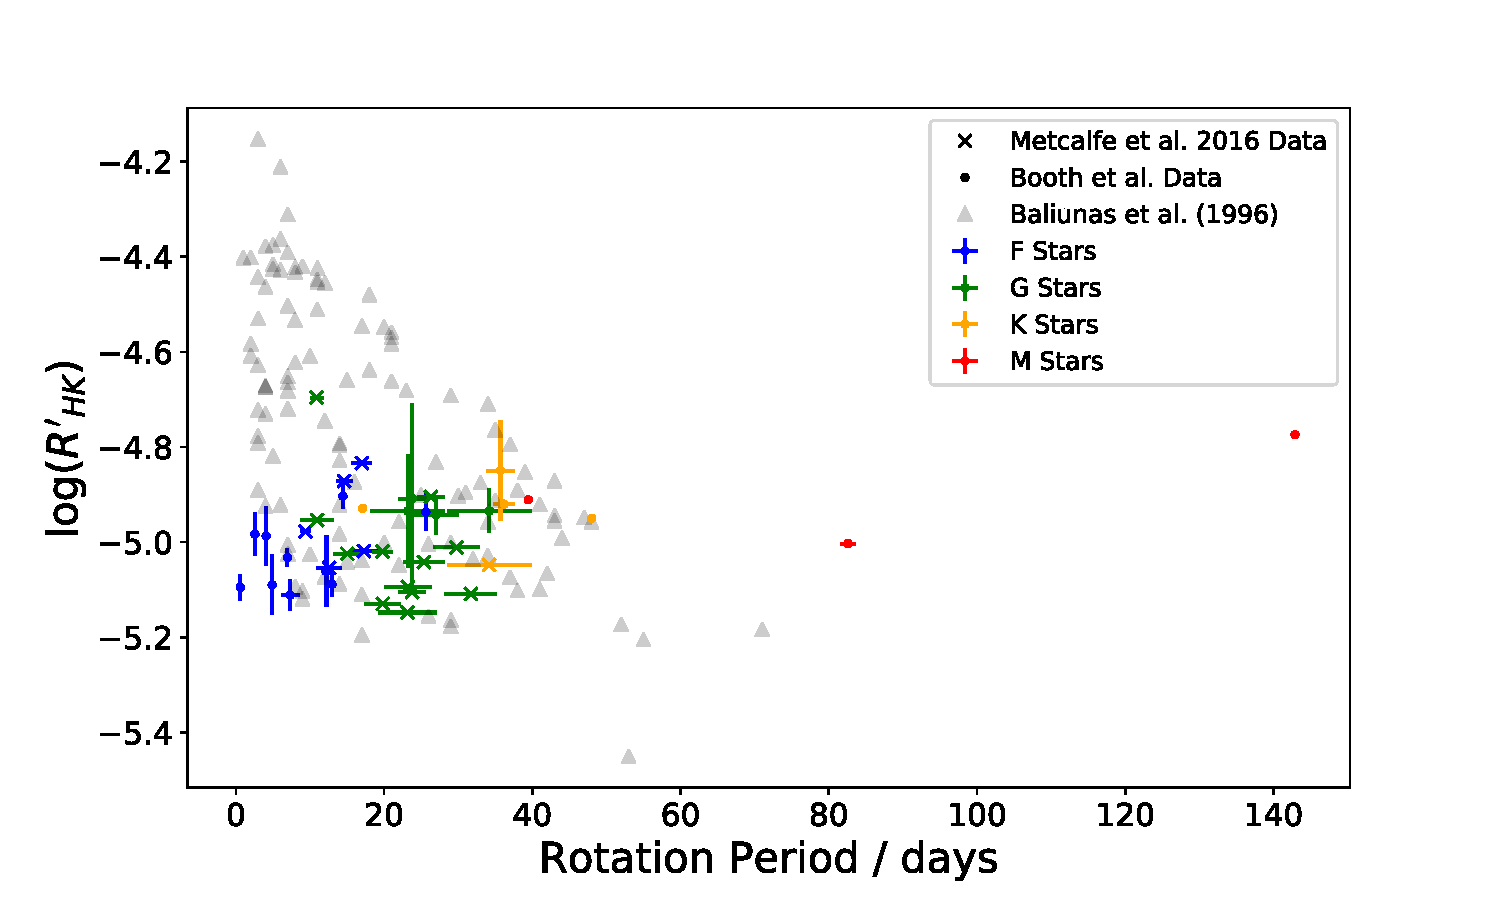
\includegraphics[width=0.95\textwidth]{Figures/5-Activity_rotation/Rhk_v_prot.pdf}
    \caption[\Rprime indicator as a function of rotation period]{Plot of the \Rprime indicator as a function of rotation period. Stars from \citet{Metcalfe_etal_2016} and this work are divided into the relevant spectral type.}
    \label{fig:rhk_v_rot}
\end{figure}

In total, 21 stars in my sample had values for the \Rprime indicator. In addition to this, data from M16 were used to compare with and complement the stars from the calcium and X-ray studies. Data from B96 was also used to place the sample of old, slowly rotating stars with known ages into context.

Figure \ref{fig:rhk_v_rot} shows the \Rprime activity indicator as a function of rotation period for the sample of stars considered in this work. Stars from B96, M16 and my sample of stars are denoted by triangle, cross and circle symbols, respectively. Furthermore, the M16 data and the sample of stars considered in this work are presented by spectral type; F--type stars are shown in blue, G--type stars in green, K--type stars in orange and M--type stars in red. Figure \ref{fig:rhk_v_rot} shows that, as expected, there is significant scatter in the rotation period for a given activity level. Calculating the Pearson coefficient for the B96 sample gives a value of $-0.59$, indicating that there is a negative correlation between the two parameters but they are not perfectly anti-correlated. The sample of stars from this work and M16 also follow a similar trend and generally agree with the B96 sample. The exception to this is the M-type stars that have extremely long rotation periods, which is to be expected since they stay on the main sequence for much longer than FGK--type stars and therefore have much longer spin-down timescales.

\begin{figure}
    \centering
    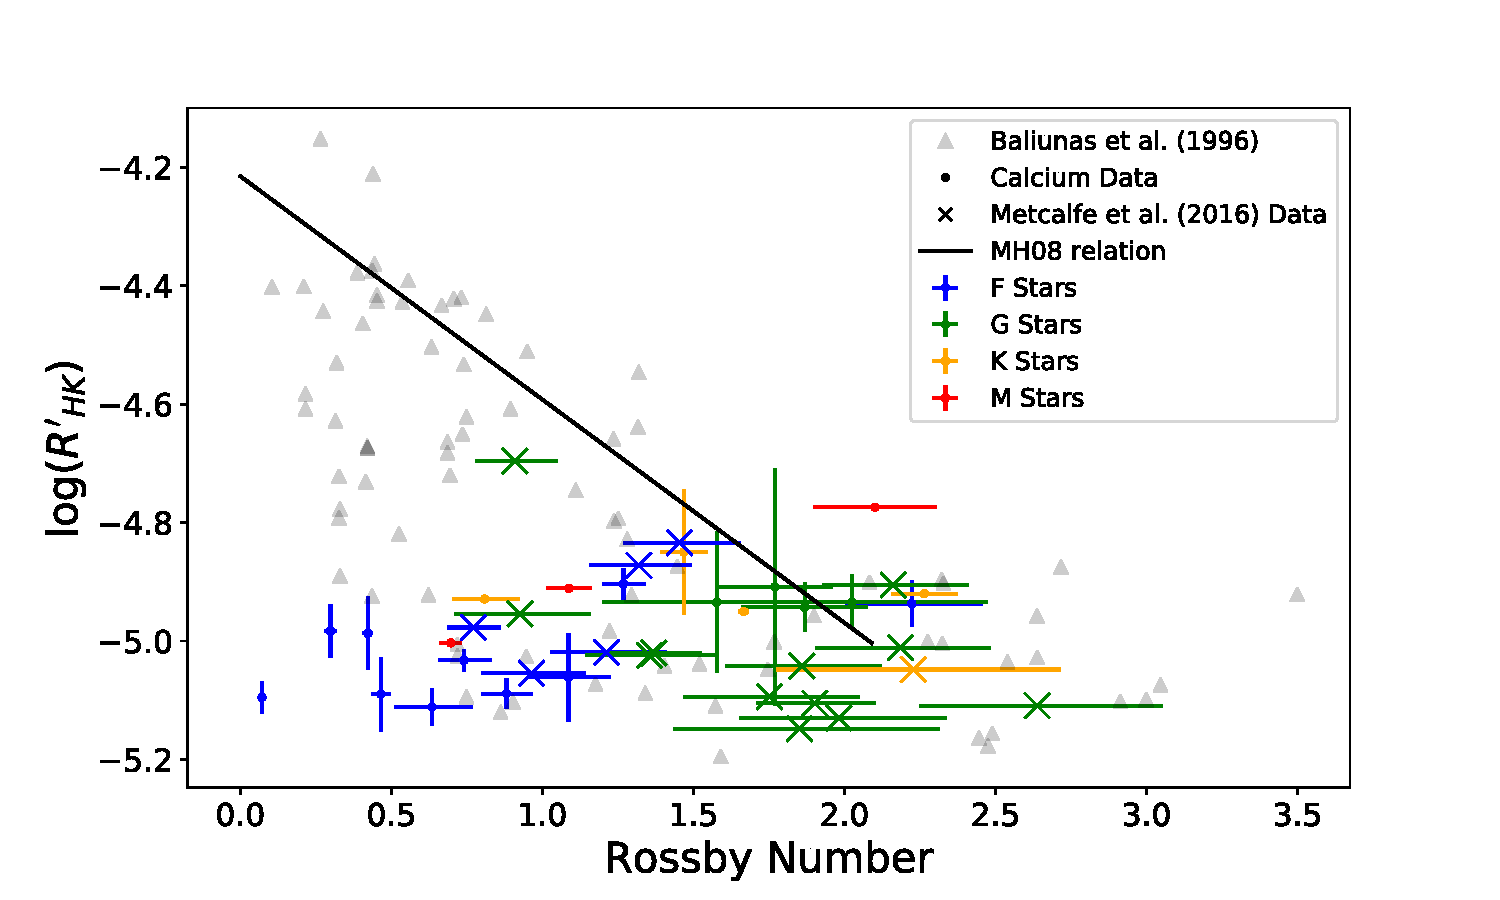
\includegraphics[width=0.95\textwidth]{Figures/5-Activity_rotation/rhk_v_r0.pdf}
    \caption[\Rprime indicator as a function of \Ro]{Plot of the \Rprime indicator as a function of \Ro. The activity--rotation relationship from \citet{Mamajek_Hillenbrand_2008} is shown in black for reference.}
    \label{fig:rhk_v_ro}
\end{figure}

In line with previous activity--rotation studies \citep{Mamajek_Hillenbrand_2008,Metcalfe_etal_2016} we consider the Rossby number instead of rotation period, as shown in Figure \ref{fig:rhk_v_ro}. Note that in order to calculate \Ro for the B96 sample, the sample was limited to $B-V < 0.77$ as discussed in Section \ref{Chp5_method}. As expected, the Pearson coefficient value of $-0.66$ shows a stronger negative correlation between the \Rprime indicator and \Ro for the limited B96 sample of stars. Despite the use of \Ro, there is still a significant spread in \Ro for a given activity level, particularly for low activity levels. It is worth noting that the F--type stars in the sample also tend to be spinning faster than one would expect from the B96 sample.

Figure \ref{fig:rhk_v_ro} also shows the activity--rotation relationship from \citet{Mamajek_Hillenbrand_2008} (MH08) for comparison. This relationship is valid in the range $-5.0 < \log(R^{'}_{HK}) < -4.3$. The MH08 activity--rotation relationship seems to describe the high activity level for a given Rossby number fairly well. However, there are many lower activity stars that cannot be accurately described by the MH08 relationship. There could be several reasons for this; one possibility is that the MH08 relationship is biased towards more active stars that have detectable light curve modulation due to starspots. Alternatively, as discussed in Section \ref{Chp4_discussion}, the stellar metallicity has an effect on the value of the \Rprime indicator calculated, therefore it could be possible that some of this scatter in \Ro for a given activity level is due to metallicity effects.


\subsection{Rotation--age}
\label{Chp5_results_rotation_age}
The collection of literature rotation periods for the sample of stars from the X-ray and calcium emission studies also gives the opportunity to investigate the rotation--age relationship. In total, 29 stars from the calcium and X-ray studies have literature rotation periods that are shown in Figure \ref{fig:full_sample_prot_v_age} alongside additional data from M16. Since stellar spin-down is inherently dependent on the mass of the star, the sample was divided into the relevant spectral types for further investigation.

\begin{figure}
    \centering
    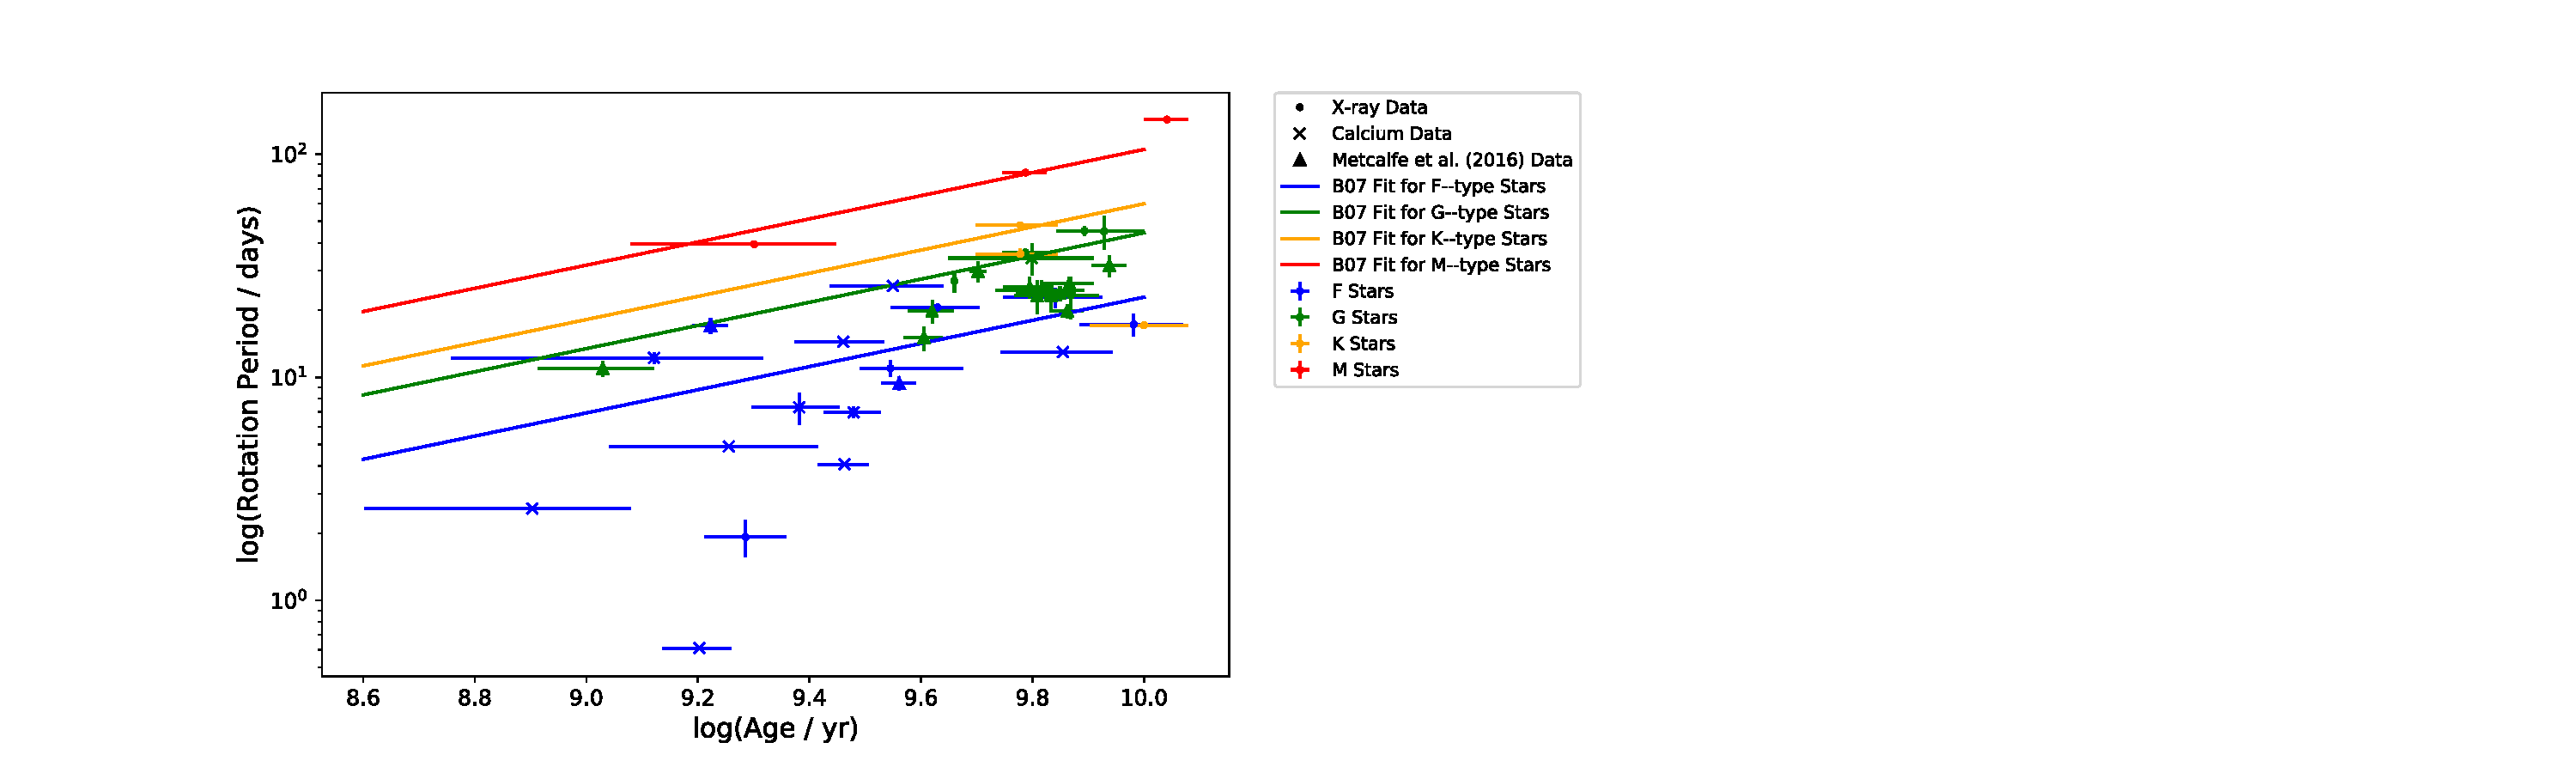
\includegraphics[width=0.95\textwidth]{Figures/5-Activity_rotation/prot_v_age_with_B07.pdf}
    \caption[Rotation period as a function of age for full sample]{Logarithmic plot of rotation period as a function of age for our sample of stars alongside additional data from \citet{Metcalfe_etal_2016}. Stars are displayed by spectral type with the marker denoting the source of the data. For each spectral type, the age--activity relationship from \citet{Barnes_2007} for the average $B-V$ colour of the sample is also plotted.}
    \label{fig:full_sample_prot_v_age}
\end{figure}

For each spectral type, the average $B-V$ colour was calculated and used to determine the rotation--age relationship from \citet{Barnes_2007} (B07). These rotation--age relationships are plotted in Figure \ref{fig:full_sample_prot_v_age} in the appropriate colour for each spectral type. It should be noted that the B07 relationship has an age exponent of 0.52, similar to the Skumanich law. The B07 rotation--age relationships seem to show reasonable agreement with the stars in each spectral type sample. However, there tends to be some stars that are spinning faster than expected from the B07 relationship, particularly in the F-- and G--type stars.

This discrepancy is highlighted when best-fitting relationships are found for the F-- and G--type stars. Note that due to the small number of K-- and M--type stars in the sample, best-fitting relationships are not found for these spectral types. The preferential method of obtaining a best-fitting relationship is to perform an ODR (orthogonal distance regression) to the data, as this method considers errors in both the x and y values. However, due to the small errors associated with the rotation period for the F--type stars in the sample, the ODR fit found a best-fitting relationship that had large uncertainties in both the gradient and y--intercept. Therefore, for this sample of stars, a linear regression was used. While the linear regression fit does not take into account the errors associated with the parameters, it gives a much more reasonable best--fitting relationship than the ODR method for this particular sample of stars. The best--fitting relationship for the F stars is shown in Equation \ref{Eq:f_stars_lin_reg}, where $t$ is the stellar age in years.

\begin{equation}
    \log(P_{rot}) = (0.91 \pm 0.33)\log(t) -7.69
    \label{Eq:f_stars_lin_reg}
\end{equation}

The best-fitting relationship as found by the ODR method is shown in Equation \ref{Eq:g_stars_ODR} for the G--type stars. Equations \ref{Eq:f_stars_lin_reg} and \ref{Eq:g_stars_ODR} show that the age exponents are steeper than the corresponding value in the B07 relationship. This highlights the discrepancy between the faster rotators in our sample and the B07 relationship.

\begin{equation}
    \log(P_{rot}) = (0.86 \pm 0.19)\log(t) - (7.00 \pm 1.84)
    \label{Eq:g_stars_ODR}
\end{equation}

\section{Discussion}
\label{Chp5_discussion}

The sample of stars considered in this work has been compared to previous activity--rotation samples and a rotation--age relationship. Here, I will discuss the potential insights that the sample has given us in context of recent age--activity--rotation relationships.

Firstly, the rotation--age analysis: showed that there was general agreement between the B07 relationship and the slower rotators in the sample. However, with the inclusion of the faster rotators, this lead to best-fitting relationships for the F-- and G--type stars that had larger age exponents ($0.91 \pm 0.33$ and $0.86 \pm 0.19$, respectively) than the Skumanich law and B07 relationship. This can be interpreted in two ways. If the activity--rotation relationship is slightly steeper, as reported by W11, then this could explain the increase in age exponent. Alternatively, if there are biases in the rotation period towards faster rotators, then this could also explain the discrepancy.

The relationship between the \Rprime indicator and rotation shows that most of the sample considered in this work is in agreement, although due to the metallicity effects on the value of the \Rprime indicator, it may not be the ideal magnetic activity indicator to use to investigate the activity--rotation relationship.

When considering the X-ray luminosity--rotation relationship, there is general agreement between the W1 sample and my sample of stars. My sample of stars lies in the lower activity area of the scatter in the relationship, which is to be expected given their ages and activity. This may also give some evidence towards the slightly steeper value of $\beta$ found in W11 of $-2.70$, but given the small sample this cannot be confirmed. In any case, the general agreement between my sample and the W11 sample shows that there is no significant steepening of the activity--rotation relationship and that these two quantities are still inherently linked. However, \citet{van_Saders_etal_2016} and the work I presented in chapter \ref{Chapter3} \citep{Booth_etal_2017} show seemingly opposite trends for the magnetic activity and rotation periods with age for samples of old, inactive stars. \citet{Booth_etal_2017} finds a steepening of the age--activity relationship, while \citet{van_Saders_etal_2016} found that older stars seemed to be rotating faster than expected from previous gyrochronology relationships, and they interpreted this as weakened magnetic braking.

There are several ways to explain the discrepancy between the two studies: One explanation is that there is a physical change that occurs within the star that causes the discrepancy between magnetic activity and rotation at these older ages. As discussed in Section \ref{Chp4_discus_spindown_context}, one potential mechanism would for older stars to undergo a change in magnetic field topology that causes the star to undergo weakened magnetic braking. However, such a physical change should be seen as a steepening in the activity--rotation relationship. The sample considered in this work was in general agreement with previous activity--rotation samples. Therefore, this casts doubt on a physical change occurring in these older stars. 

Another plausible explanation is that there are biases in the stellar samples being considered in the studies. I acknowledged this in the X-ray luminosity study \citep{Booth_etal_2017} and considered the X-ray luminosity through the stellar surface area to account for the mass bias seen in the X-ray luminosity. Also, determining upper limits for the X-ray luminosity is relatively straightforward through the use of photon statistics. Therefore, we can detect when a star has a very low level of stellar activity. However, when considering rotation periods, it has now come to light from the work by \citet{van_Saders_etal_2019}, that there is a Rossby number "edge" of value $2.08$, above which long period, high Rossby number stars are either not detectable or are simply absent. This value for the Rossby number edge is comparable to that \citet{van_Saders_etal_2016} found for the critical Rossby number, above which it was theorised that weakened magnetic braking occurred. Therefore, to determine whether long period, high Rossby number stars exist, alternative methods of determining the rotation period must be used. One alternative method is to use the periodic variation in magnetic activity indicators such as the \Rprime indicator, which is commonly used in determining rotation periods of slow rotators.

Finally, it has been noted in this analysis that the F--type stars seem to lie below the previous activity--rotation samples. It is possible that these stars don't quite follow the activity--rotation relationship due to their thin convective zones. This would have to be confirmed with a larger sample of F--type stars with determined rotation periods, but it may explain the discrepancy between \citet{Booth_etal_2017} and \citet{van_Saders_etal_2016}. The study by \citet{van_Saders_etal_2016} had a majority of F--type stars in their sample; this, combined with potential biases towards faster rotators from periodic variations in light curves, may explain the faster rotation periods at older ages.


\section{Conclusions}
In this work, rotation periods were collected for 29 old, inactive stars that I previously studied in Chapters \ref{Chapter3} and \ref{Chapter4}. One of the possible causes for the steepening of the age--activity relationship observed in Chapter \ref{Chapter3} was a change in the activity--rotation relationship for older stars. Therefore, the activity--rotation relationship was investigated using the rotation periods collected from the literature. With the collection of literature rotation periods, the rotation--age relationship was also investigated. General agreement was found between the sample of stars in this work and the B07 rotation--age relationship. However, age exponents were found for the best-fitting relationships for the F-- and G--type stars that were larger than that of the B07 relationship. This may be due to a slight steepening of the activity--rotation relationship (as reported by W11) or due to potential biases in the rotation periods collected from the literature. The \Rprime--\Ro plot showed significant scatter for the sample considered; this could be a combination of mass and metallicity effects in the \Rprime activity indicator.

When considering the X-ray luminosity as the activity indicator for the activity--rotation relationship, the sample of stars seem to be in agreement with a previous sample of stars \citep{Wright_etal_2011}. The X-ray luminosity--rotation relationship shows that there is no significant steepening of the relationship as suggested by \citet{Booth_etal_2017}. This evidence would cast doubt on any potential physical change in the stars as an explanation for the discrepancy between magnetic activity and rotation at older ages, as this would be seen in the activity--rotation relationship. Therefore, alternative methods for determining the rotation period must be used in attempt to prove if the Rossby "edge" shown in \citet{van_Saders_etal_2019} is due to stars being undetected or if it has a basis in real physical processes. Lastly, the discrepancy between the F--type stars in the sample considered in this work and previous activity--age samples may hint that these stars do not follow the activity--rotation as closely as the rest of the stars in the sample. If confirmed, this may provide an alternative explanation for the discrepancy between magnetic activity and rotation periods for older main sequence stars.

Further studies combining age, activity and rotation will improve the sample considered in this work and help shed light on the the possible processes at work in these older stars.